%----------------------------------------------------------------------------
\section{Arclenyomatok adatvédelmi elemzése}
\label{sec:4}

%--------------------------------------------------------------------------------------------------
\subsection{Támadó modellezése}  % 1 oldal
% - Támadómodell bemutatás (copy ábra Gábortól, lényeget leír)
% - Jelenlegi arcfelismerő rendszerek sebezhetősége, hogyan férhet hozzá
% - Feltételezzük, hogy a támadó interneten elérhető datasetekhez hozzájut ami alapján betanít classifiert és ezt használva tud kinyerni adatot. Következő fejezetben erre mutatunk példát hogyan lehetséges

A következőkben az arcfelismerő rendszerek sebezhetőségét fogom elemezni. Az arcfelismerő rendszerek általános működését a [REF] fejezetben korábban bemutattam. Az adatvédelmi elemzéshez szükséges definiálnom egy támadó modellt. Tegyük fel, hogy egy cégnél alkalmaznak arcfelismerő rendszert a dolgozók azonosítására. Az épület számos helyisége be le van fedve CCTV térfigyelő kamerákkal, amelyek egy központi arcfelismerő rendszernek továbbítják a felvételeket. Új dolgozó regisztrációja során az arcfelismerő rendszer néhány felvétel alapján kiszámolja a dolgozó arcát lebjobban leíró arclenyomatát, amit egy központi szerveren tárol. Miután a dolgozó arclenyomata szerepel az adatbázisban, a térfigyelő kamera felvételek alapján lehetséges őt azonosítani. Egy ilyen arcfelismerő rendszernek a főbb részei: 

% TODO ide lehet szoftver példákat hozni ha kell content
% magyar szavakat kéne használni
\begin{enumerate}
	\item Kamera rendszer: amely a nyers képkockákat továbbítja az adatfeldolgozó egységnek
	\item Feature extractor: amely az egyes kékkockákon végzi a gyorsan lefuttatható arcdetektálást. Ha sikeresen talál emberi arcot az egyik kékkockán, arra elvégzi az arc geometriai transzformációját, majd az arcból kinyeri az arclenyomatot.
	\item Adatbázis: Az ismert, címkézett arclenyomatok tárolására szolgál.
	\item Matcher: A kinyert arclenyomatot összehasonlítja az adatbázisban tárolt dolgozók arclenyomataival, majd azokon valamilyen távolság (pl: Euklideszi távolság) metrika alapján megállapítja a legvalószínűbb találatot. Ha a legkisebb távolság egy bizonyos küszöbértéknél kisebb, akkor a dolgozót sikeresen azonosította, ellentkező esetben ismeretlen személynek nyilvánítja.
\end{enumerate}

Míg az ilyen arcfelismerő rendszer több módon is támadható, a dolgozatom során azzal az esettel foglalkozom, hogy a rosszindulatú fél valamilyen módon hozzáférést nyer az arclenyomat adathalmazhoz, ami lehet egy belső alkalmazott aki kiszivárogtatja az adatbázist, vagy akár egy külső támadó, például hacker aki sikeresen feltöri rendszert. Előfordulhat, hogy a támadó az adatbázisnak egy kisebb részéhez fér hozzá, de dolgozatom során a legerősebb támadót feltételezem, aki a teljes adatbázishoz hozzáfér, illetve feltételezem, hogy az arclenyomatok titkosítás nélkül vannak tárolva a szerveren.

% TODO saját ábra?
\begin{figure}[ht]
	\centering
	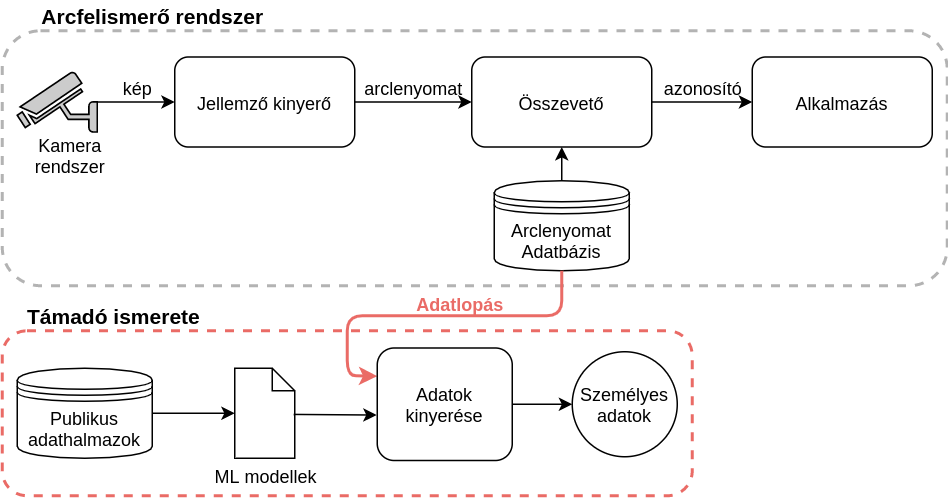
\includegraphics[width=1\columnwidth]{figures/attacker_model.png}
	\caption{ideiglenes ábra}
	\label{fig:attacker}
\end{figure}

A támadó modellezését a \ref{fig:attacker}. ábra mutatja be. Miután a támadó valamilyen módon hozzáférést szerzett a központi szerverhez, amin az arclenyomatok vannak tárolva, elképzelhető, hogy képes lesz az arclenyomatokból személyes adatokat kinyerni az adatalanyokról. Személyes adatnak minősül bármilyen adat, ha közvetlenül beazonosítható általa az érintett személy (közvetlen azonosítók), vagy ha közvetetten (kvázi-azonosítók) \cite{GDPR2018}. Személyes adat lehet például a személy demográfiai adatai, mint például a személy életkora, a neme, vagy a rassza. 

Feltételezhetjük, hogy a támadó a személyes adatok kinyeréséhez egy saját fejlesztésű algoritmust használ, ami lehet például egy gépi tanulási modell is. Ha a támadó képes megfelelően nagy valószínűséggel, megbízható módon kinyerni a személyes adatokat, akkor a támadó feltételezheti, hogy a kinyert adatok valósak. A sikeresen kinyert adatokat majd saját célból fel tudja használni a támadó, például újraazonosításos támadáshoz. A személyes adatok kiszivárgásának adatvédelmi kockázatait a [REF]. fejezetben fejtem ki bővebben.

A kérdés az, hogy milyen eljárással lehetséges egy arclenyomatból kinyerni az adatalan érzékeny információit? A munkám során erre a kérdésre kerestem választ. Feltételezésem az volt, hogy az interneten ingyenesen, publikusan elérhető emberi arcokról készült fotókból összeállítható egy nagy méretű adathalmaz, amihez rendelkezésre állnak a fotón látható valamennyi személy demográfiai adatai, például a pontos vagy becsült életkora, neme és rassza, vagy bármilyen adat ami fotó alapján ember által megadható, és később segíthet az illető azonosításában. Ha sikerül egy ilyen adathalmazt összeállítani, akkor az arcképek alapján az arcfelismerő rendszer működéséhez hasonlóan minden arcképről generálhatunk arclenyomatokat. Ezt követően rendelkezünk az arclenyomatokkal, és a hozzájuk tartozó címkékkel.

Miután megvan az arclenyomat adathalmaz, az alapján képesek vagyunk betanítani egy gépi tanulási modellt, ami az arclenyomatok és a hozzájuk tartozó címkék alapján képes tanulni. A betanítás után a modell használható arra, hogy új, nem látott arclenyomat mintákra becslést adjon. Visszatérve a támadóhoz, ha a támadó rendelkezik egy előre betanított gépi tanulási modellel, azt felhasználhatjra arra, hogy a szerverről szerzett arclenyomat adatbázisból érzékeny adatokat nyerjen ki. 

A támadó sikerességének feltétele az, hogy képes hozzáférni a szerveren tárolt arclenyomatokhoz, illetve az, hogy a gépi tanulási modellje milyen megbízhatósággal képes becslést hozni a személyes adatokra. A két feltétel közül a másodikkal foglalkozom a továbbiakban. Azt vizsgáltam, hogy modern tanuló algoritmusokkal milyen eredmény érhető el.

%--------------------------------------------------------------------------------------------------
\subsection{Adathalmazok}  % 3-4 oldal

Első lépésként szükségem volt egy megfelelően felcímkézett arclenyomat adathalmazra. Ezt az adathalmazt használom fel arra, hogy az alapján tanítsak be gépi tanulási modelleket, amelyek majd képesek becslést adni személyes adatokra. Egy-egy modell csak egy személyes adatra tud becslést adni, ezért több modellre van szükség. Célom az volt, hogy személyes adatok közül az illető életkorát, nemét és rasszát becsüljem meg. Ehhez szükséges tanító mintakészlet, amiben az életkor, nem és rassz meg van címkézve. Elvárás volt még az is, az arclenyomat adathalmazban minden személynek saját azonosító címkéje legyen, illetve lehetőleg minél több arclenyomat tartozzon egy-egy személyhez. Erre azért van szükség, mert az arclenyomatokon vizsgáltam az identifikációs modell teljesítőképességét is. 

Mivel a feladatból adódóan az adathalmazzal szemben támasztott elvárások eléggé specifikusak, ezért szükség volt saját adathalmaz létrehozására. Azért, hogy meggyorsítsam a munkámat, kiindulásnak kerestem olyan online elérhető, arcképeket tartalmazó adathalmazt, ami már előre fel van címkézve. Ha létezik egy megflelő arckép adathalmaz, akkor a képekből egyessével kinyerhetőek az arclenyomat vektorok. 

Az arckép adathalmazzal szemben az elvárások a következők:
\begin{itemize}
	\item Lehetőleg kutatási célra lettek létrehozva, az enyémhez hasonló feladatra. Ennek megfelelően az arcképek már előre vannak készítve a feldolgozáshoz (pl. arc kivágása a képből).
	\item Az adathalmaznak megfelelően nagynak kell lennie ahhoz, hogy gépi tanulási modellt sikeresen be lehessen tanítani róla.
	\item Egy emberről lehetőleg minél több kép legyen ahhoz, hogy a generált arclenyomatok alapján identifikáció jól működjön. Minél több képünk van egy illetőről, anál biztosabban lehet meghatározni az ember arcát legjobban leíró arclenyomatot.
	\item A képek megfelelő demográfiai adatokkal vannak címkézve. Esetemben a szükséges címkék: az életkor, nem és a rassz.
\end{itemize}

Nehéz olyan adathalmazt találni, amiben mindhárom számunkra fontos demográfiai adat szerepel. Több arckép adathalmaz jónak tűnt elsőre, de az elvárások közül nem felelt meg egynek. Néhány ilyen adathalmaz amivel foglalkoztam: Labled Faces in the Wild \cite{labledfacesinthewild2008}, Face Image Project \cite{faceimageproject2014}, CelebA \cite{celebA2015}. A FairFace \cite{fairface2021} egy viszonylag új adathalmaz, ami nagyon igéretesnek tűnt, mert mindhárom demográfiai adatot tartalmazza, és az egyes osztályok aránya kiegyensúlyozott, viszont nem tartalmaz identifikációs címkét.

Végül nem sikerült olyan adathalmazt találnom ami minden kritériumnak megfelel, ezért két külön adathalmazt használtam fel. Az egyik a VGGFace2 \cite{vggface22018} amit rassz és nem becslésére használtam fel, a másik pedig az IMDB-WIKI dataset \cite{imdbwiki2018}, amit életkor becsléshez használtam fel. A két választott arckép adathalmazt szükség volt feldolgozni ahhoz, hogy azokból gépi tanulási modellt lehessen tanítani. A feldolgozás menetét mutatom be a következő részekben.

\subsubsection*{VGGFace2 adathalmaz}

Jelenleg az egyik legnagyobb publikusan elérhető, kutatási célra készült arckép adathalmaz a VGGFace2. Az adathalmaz 3,31 millió arcképet tartalmaz mindössze 9131 emberről, átlagosan 362,6 kép mindenkiről. A képeket a Google képkeresőjével gyűjtötték össze. Az adathalmaz képein sokféle ember szerepel, eltérő demográfiai adatokkal és eltérő szakmával (pl. vannak színészek, sportolók, politikusok). A képeken látható emberek többféle pózban láthatóak, sokféle megvilágításban. Az összegyűjtött képeket automatikusan és manuálisan is szűrték.

A VGGFace2 alapból nem tartalmaz rassz címkéket, viszont a Salernói Egyetem MIVIA kutatócsoportja manuálisan felcímkézte az adathalmazt rassz címkékkel, és a munkájukat publikusan elérhetővé tették VMER névvel \cite{vmer2020}. A VMER-rel kiegészítve a VGGFace2 címkéit, így már van rassz, nem és identifikációs címke is az összes mintához.

Az arcképeket egyesével dolgozza fel egy script, ami az arcképekből kinyeri az arclenyomatokat. Ehhez a face\_recognition Python könyvtárat \cite{face_recognition} használtam fel, ami a [REF sec:problema]. fejezetben taglalt módon találja meg, és alakítja át a képen látható arcokat arclenyomattá. Az arclenyomatok kinyeréséhez a dlib-et \cite{dlib2009} használja, így a kapott arclenyomatok 128 dimenziós lebegőpontos vektorok lesznek. Az adathalmazban előfordulnak olyan képek, ahol több ember arca is látható, (például a háttérben elsétál valaki). Ez problémás, mivel ilyenkor nem egyértelmű, hogy a képen látható melyik archoz tartozik az annotáció. E miatt a scriptem csak olyan képekkel foglalkozott, ahol pontosan egy arcot sikerült azonosítani. A script-ből egy függvény látható a \ref{lst:get_encoding}. kódrészleten.

\begin{lstlisting}[language=python, caption={Arclenyomat vektorok kinyerése.}, label=lst:get_encoding]
def get_encoding(filepath):
  # kep beolvasasa
  image = face_recognition.load_image_file(filepath) 
  # arcok detektalasa 
  face_locations = face_recognition.face_locations(image,
    number_of_times_to_upsample=1, model="cnn")
  if (len(face_locations) == 1): 
    # arclenyomat vektor
    return np.array(face_recognition.face_encodings(image,face_locations))[1]
  return None
\end{lstlisting}


Mivel 3,3 millió arcképet kellett feldolgozni, a Python scriptet Google Colab-en futtattam, aminek az az előnye, hogy ingyenesen lehet használni korszerű GPU-kat, illetve az adathalmaz feldarabolásával párhuzamosan több session-t is lehet futtatni, jelentősen felgyorsítja a képek feldolgozását.

A következő lépés az adathalmaz tisztisása volt, azaz kiszűrni azokat a képeket, amelyek valamilyen okból rossz minőségűek (például távoli fotó, rossz fényviszony vagy fura szögből készült a kép), vagy az illető a többi képhez képest nagyon eltérően néz ki. Az arclenyomatok szűréséhez minden személyhez kiszámítottam az átlagos arclenyomatot (centroid), és a centroidtól vett távolság alapján a túl nagy távolságra lévő arclenyomatokat szűrtem az adathalmazból. 

A feldolgozás és szűrés után kapott adathalmaz közel 3 millió arclenyomatot tartalmaz. Minden arclenyomathoz tartozik egy ID címke ami azonosítja az képen látható személyt. Egy ID-hoz legalább 50 arclenyomat tartozik. E mellett van még nem címke (férfi, nő), és rassz címke (African American, East Asian, Caucasian Latin, Asian Indian). Ekkor probléma volt az, hogy az egyes osztályokhoz sokkal több minta tartozott mint más osztályokhoz. A leggyakoribb a fehér férfiak aránya volt, míg a legritkább az afroamerikai nők. Az osztályok arányát a \ref{fig:vgg_imba}. ábra mutatja be.

\begin{figure}[ht]
	\centering
	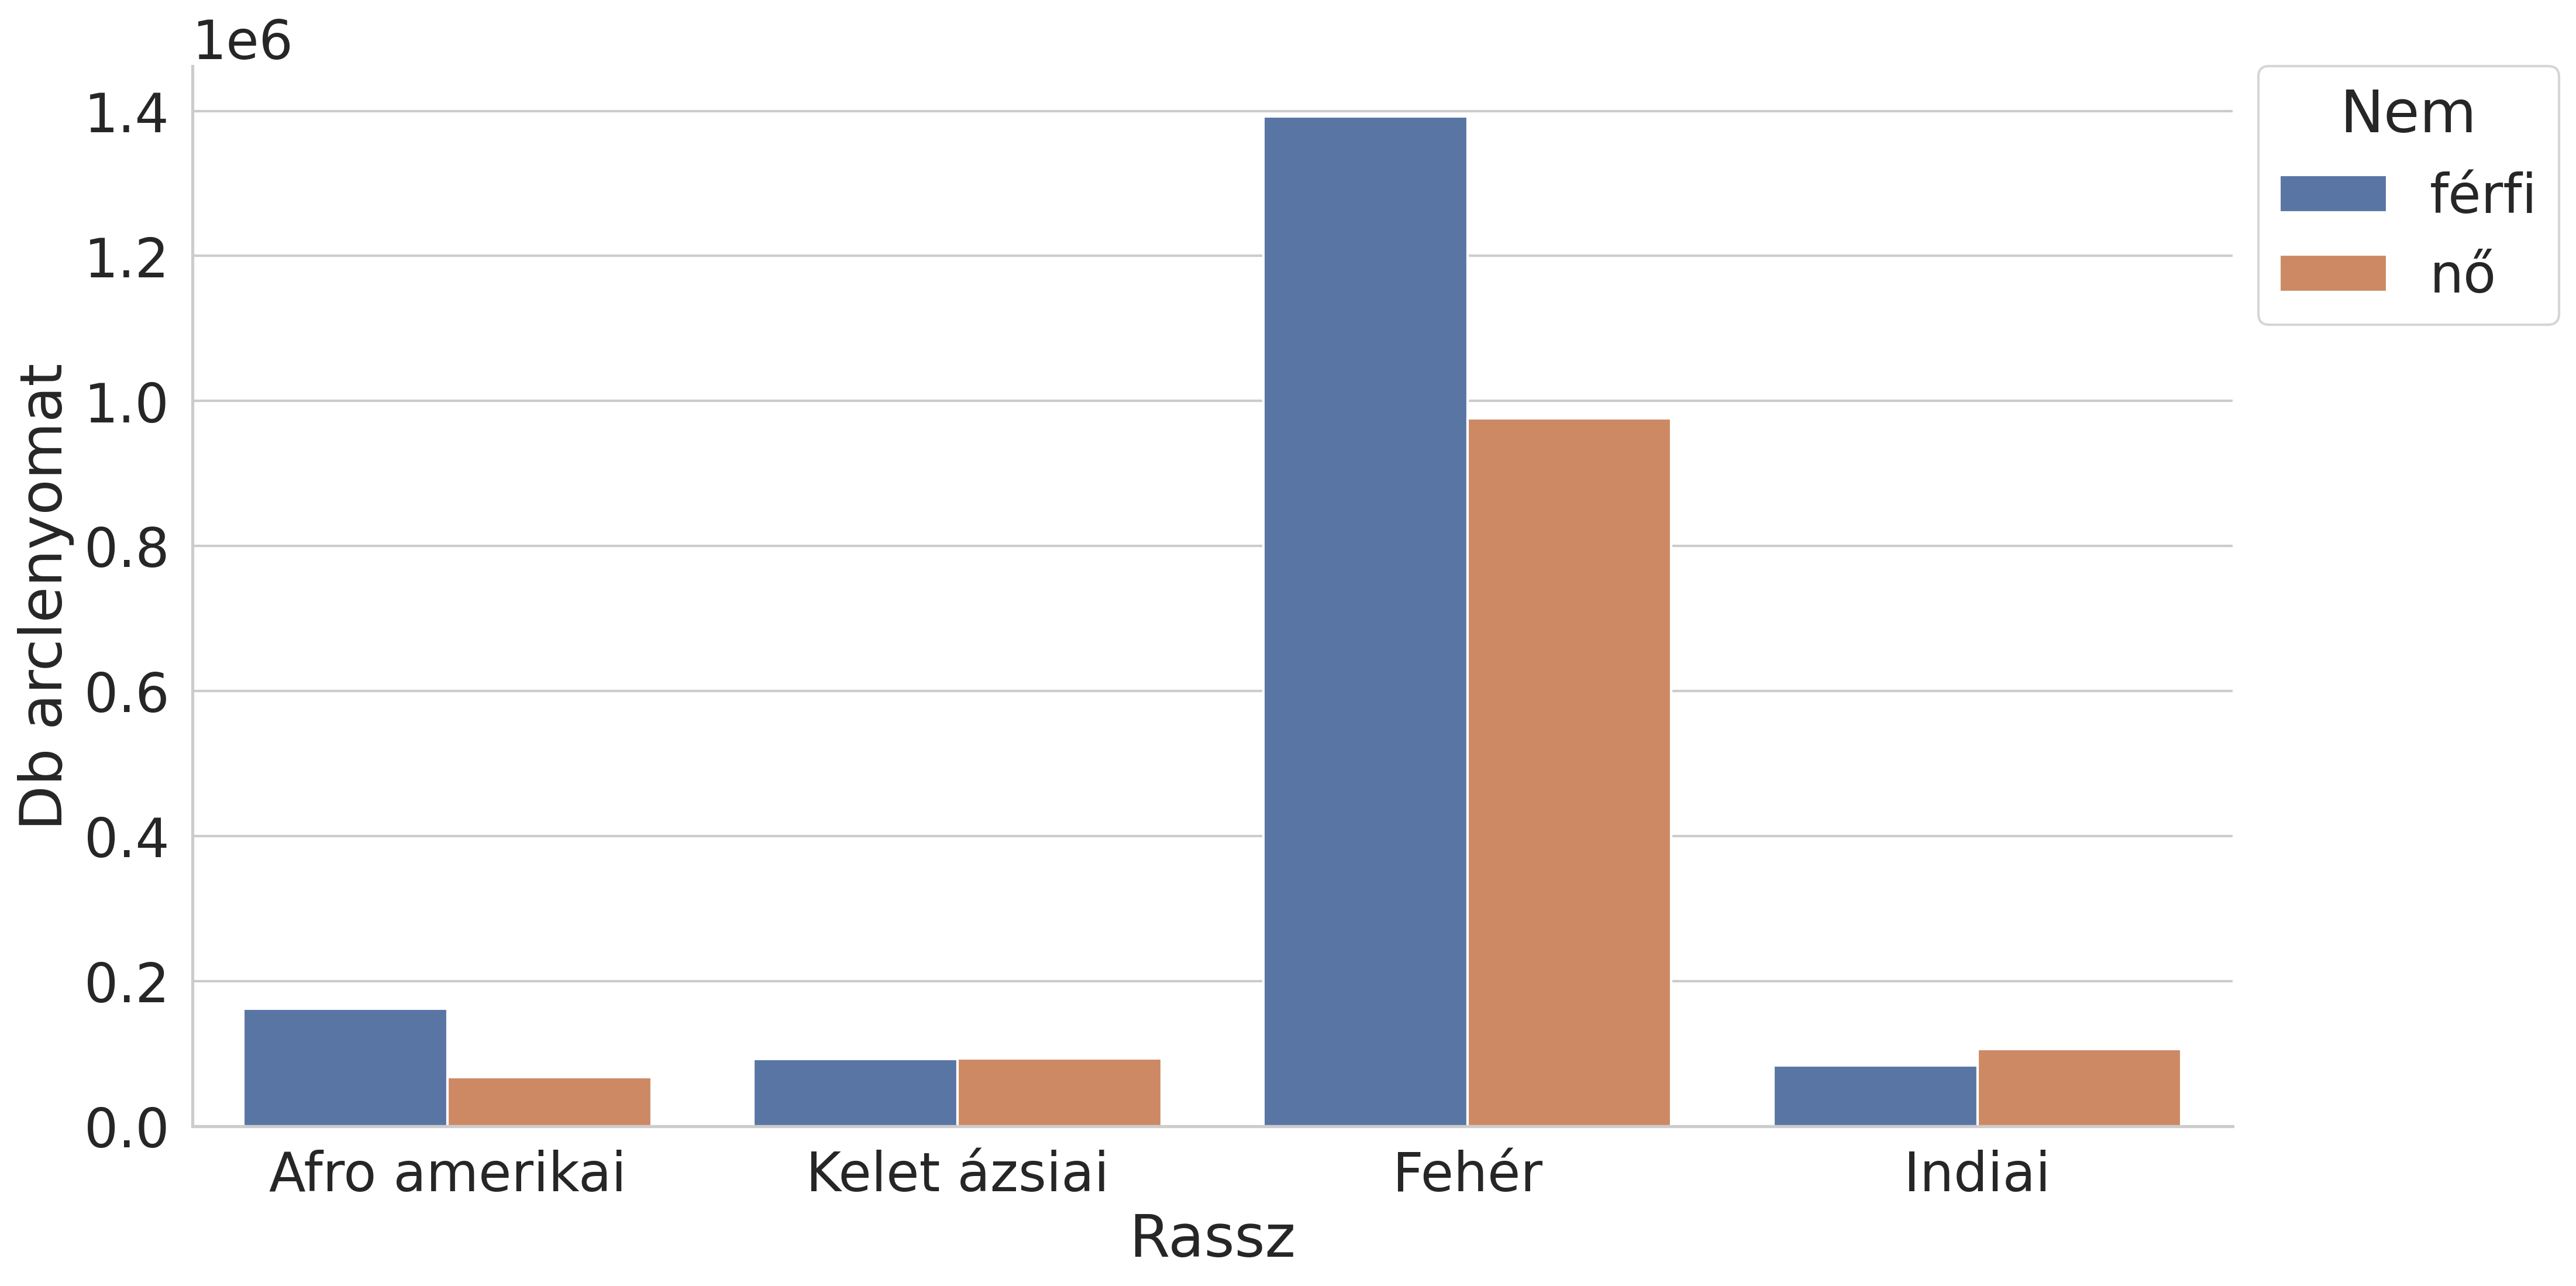
\includegraphics[width=1\columnwidth]{figures/VGG_imba.png}
	\caption{Osztályok aránya az arclenyomat adathalmazban.}
	\label{fig:vgg_imba}
\end{figure}

Az osztályok eloszlásának aránytalansága problémát jelent az osztályozó modellek tanításakor, ezért szükséges volt az adathalmazt kiegyensúlyozni. Az adathalmaz kiegyensúlyozása minták eltávolításával érhető el. Legkevesebb kép az afroamerikai nőkről van az adathalmazban, ezért ehhez mérten szűkítettem a többi csoportot. Az embeddingek kivételénél fontos volt, hogy továbbra is legalább 50 kép maradjon minden személyről, ezért nem véletlenszerűen vettem ki a képeket, hanem ID-k alapján csoportosítva. Az egyes demográfiai csoportoknál kilistáztam az oda tartozó ID-kat, és egyes ID-khoz tartozó képek számát. Az ID-kat képszám szerint csökkenő sorrendben távolítottam el, amíg a csoport meg nem közelítette a szükséges méretet. Ezzel a módszerrel sikerült elérni, hogy minden rassz-nem párhoz ugyanannyi ember tartozott. A kiegyensúlyozott után az osztályok eloszlása a \ref{fig:vgg_ba}. ábrán látható.

\begin{figure}[ht]
	\centering
	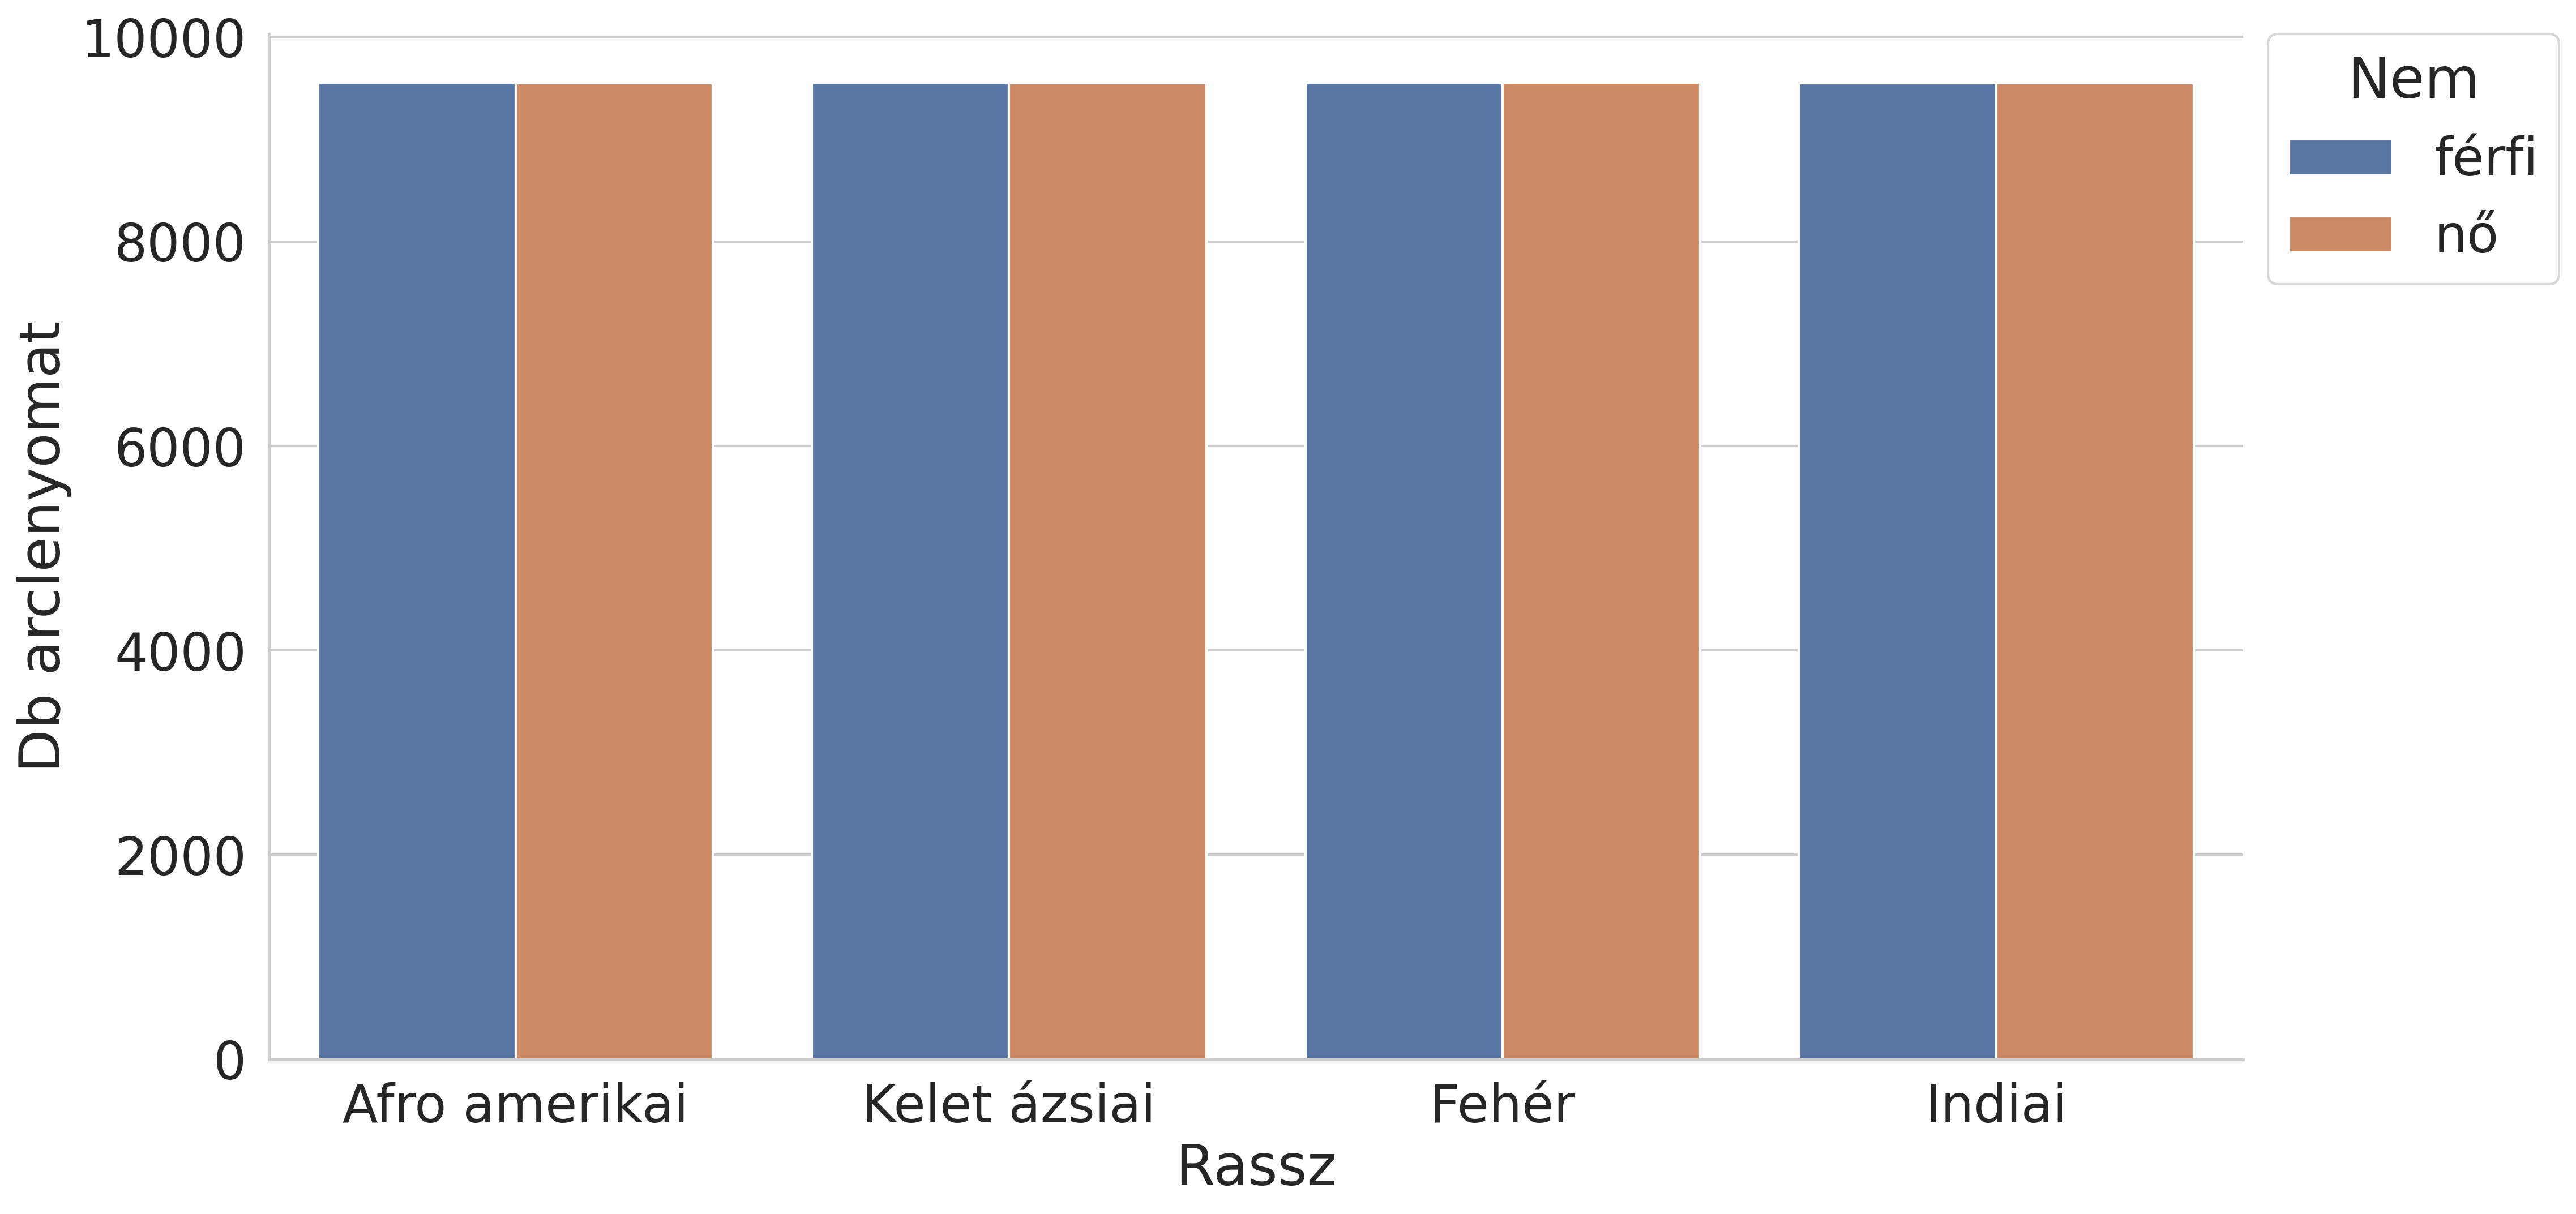
\includegraphics[width=1\columnwidth]{figures/VGG_balanced.png}
	\caption{Osztályok aránya az kiegyensúlyozás után.}
	\label{fig:vgg_ba}
\end{figure}

Az eredeti 3,3 millió képből végül 540000 arclenyomat készült, ami továbbra is nagy adathalmaznak tekinthető. Ez elegendően nagy ahhoz, hogy ez alapján osztályozó modelleket lehessen rajtuk betanítani.

\subsubsection*{IMDB-WIKI adathalmaz}

Mivel a VGGFace2 adathalmaz nem tartalmaz életkor címkét, ezért tovább folytattam a keresést. Választásom az IMDB-WIKI \cite{imdbwiki2018} adathalmazra esett. Ez az egyik legnagyobb, nyilvánosan elérhető arckép adathalmaz, ami tartalmaz azonosító címkét, nemet és életkort is. Az adathalmaz két részből áll: IMDB filmekről és filmszínészekből álló adatbázisból kinyert fotókból, illetve a Wikipédiáról szerzett fotókból. Sajnos a Wikipédiáról szerzett képekhez nem tartozik azonosító címke, így csak az IMDB-ről szerzett fotókat használtam fel.

Az IMDB-WIKI adathalmaz képekből, és hozzájuk tartozó címkékből áll. A címkék egy metadata fileban találhatóak, ami többek között tartalmazza a képen látható személy nevét, nemét, a születési dátumát, illetve azt, hogy mikor készült a fotó. A életkort a képen látható személy születési dátumából, és a kép keletkezésének dátuma alapján lehet kiszámolni. A képek jelentős része csoportkép, azaz több arc is látható rajtuk. A képek közül csak azokat használtam fel, ahol pontosan egy arcot lehetett detektálni. Továbbá, kiválasztottam azokat az azonosítókat, amihez legalább 30 fotó tartozik.

A weboldalról letölthetőek az eredeti, teljes méretű képek, illetve a már megvágott csak arcokat tartalmazó képek is. A képeken az arcok középre vannak rendezve 40\%-os ráhagyással. A képek feldolgozásánál ezért levágtam ezt a 40\%-ot, így gyorsabb a feldolgozás és jelentősen több képen sikerült arcot detektálni. Az arcokhoz tartozó képeket a VGGFace2-nél bemutatott módszerrel alakítottam át arclenyomat vektorokká.

\begin{figure}[ht]
     \centering
     \begin{subfigure}[b]{0.45\columnwidth}
         \centering
         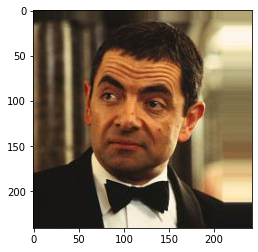
\includegraphics[width=1\columnwidth]{figures/mrbean.png}
     \end{subfigure}
     \begin{subfigure}[b]{0.45\columnwidth}
         \centering
         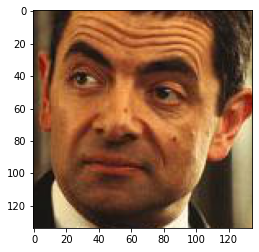
\includegraphics[width=1\columnwidth]{figures/mrbean_crop.png}
     \end{subfigure}
        \caption{Az eredeti és a megvágott kép}
\end{figure}


Az adathalmaz képeit vizsgálva azt tapasztaltam, hogy néhány fotón nem a címkének megfelelő személy szerepelt. A hibásan címkézett képek kiszűréséhez a már feldolgozott arclenyomat vektorokat használtam fel. Egy személyhez tartozó arclenyomat vektorok alapján kiszámítottam a vektorok súlypontját (centroidját), és ehhez mért Euklideszi távolságok alapján szűrtem ki a kiugró értékeket. Azt a határt, ami alatt elfogadta az arclenyomat vektor értékét 0,5-re állítottam be, ami viszonylag szigorúnak számít. Ezt az eljárást szemlélteti a \ref{lst:cent}. kódrészlet.

% TODO itt kicsit gebasz van a page break miatt
% \noindent
% \begin{minipage}{\columnwidth}
\begin{lstlisting}[language=python, caption={Arclenyomatok szűrése távolság alapján.}, label=lst:cent]
def filter(df, cutoff=0.5):
	encodings = df.iloc[:,4:].values  # egy szem(*@\color{codegreen}é@*)lyhez tartoz(*@\color{codegreen}ó@*) arclenyomatok
	centroid = np.mean(encodings, axis=0)  # s(*@\color{codegreen}ú@*)lypont sz(*@\color{codegreen}á@*)m(*@\color{codegreen}í@*)t(*@\color{codegreen}á@*)s
	distance = np.linalg.norm(encodings - centroid, axis=1)  # euklideszi t(*@\color{codegreen}á@*)vols(*@\color{codegreen}á@*)g
	return df.index[distance > cutoff]
\end{lstlisting}
% \end{minipage}

Feldolgozás után közel 90000 arclenyomat vektort kaptunk eredményül. Az adathalmazon belül a nemek aránya közel azonos, viszont az életkor eloszlása már kevésbé egyenletes (látsd: \ref{fig:agedist}. ábra). Mivel a képek az IMDB weboldalról lettek összegyűjtve, ezért főleg színészekről, filmrendezőkről vannak képek, akik tipikusan a 20-40-es életkor tartományba esnek. E miatt kiskorúakról és idős emberekről viszonylag kevés kép van az adathalmazban.

\begin{figure}[ht]
	\centering
	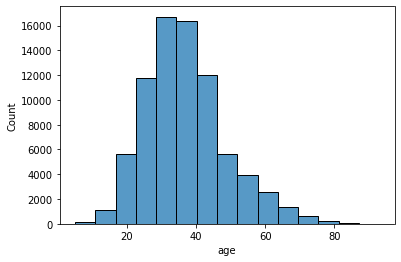
\includegraphics[width=0.7\columnwidth]{figures/IMDB_age_dist.png}
	\caption{IMDB adathalmazban az életkor eloszlása.}
	\label{fig:agedist}
\end{figure}



%--------------------------------------------------------------------------------------------------
\subsection{Modellek betanítása, eredmények}  % 1 oldal RFC, 1-2 oldl eredmények
% - RFCről röviden, miért ezt választottam, 
% - Tanítás módszeréről (használt paraméterek, modell jellemzők, age hogy lett kezelve, ID hogy lett kezelve) 
% - Betanított modellek accuracy precision, recall, F1 score, Confusion matrix, ROC curve

asdf










%--------------------------------------------------------------------------------------------------
% \subsection{Adatvédelmi elemzés}  % (1-2 oldal)
% - Adatvédelmi elemzés -> milyen riskek vannak (munkacsoport szerint) pl: több info kiderülése 1 emberről probléma, adatszivárgás: le tudja szűkíteni, hogy ki lehet az, singling out, vagy lehet arcot rekonstruálni az embeddingből, újraazonosítás.

%--------------------------------------------------------------------------------------------------



% -- PASTA --




% \begin{lstlisting}[language=python, caption=lista alatti szoveg, label=lst:Example]
% def filter(df, cutoff=0.5):
% 	encodings = df.iloc[:,4:].values  # Szem(*@\color{codegreen}é@*)lyhez tartoz(*@\color{codegreen}ó@*) arclenyomatok
% 	centroid = np.mean(encodings, axis=0)  # S(*@\color{codegreen}ú@*)lypont sz(*@\color{codegreen}á@*)m(*@\color{codegreen}í@*)t(*@\color{codegreen}á@*)s
% 	distance = np.linalg.norm(encodings - centroid, axis=1)  # Euklideszi t(*@\color{codegreen}á@*)vols(*@\color{codegreen}á@*)g
% 	return df.index[distance > cutoff]
% \end{lstlisting}


%--------------------------------------------------------------------------------------------------
% A kutatás során felhasznált adathalmaz viszonylag kis méretű, 2650 képet tartalmaz. Későbbiekben ahhoz,
% hogy meggyőződhessünk a módszereink működéséről, szükséges egy nagyobb adathalmazon is
% tesztelnünk. Ehhez olyan adathalmazra van szükségünk, ami:
% •
% •
% •
% •
% Legalább 8-10000 képből áll
% 2-3 demográfiai adattal, illetve identifikációs címkével ellátott
% Személyenként legalább 30 képet tartalmaz
% Szabadon használható, publikusan elérhető
% 8.1 VGGFace2 adathalmaz
% Nehéz olyan adathalmazt találni, amiben mindhárom, számunkra fontos demográfiai adat szerepel. A
% FairFace 18 adathalmaz ígéretesnek tűnt, de nem tartalmaz azonosító címkéket. Az egyik legnagyobb
% arcfelismeréshez készült adathalmaz a VGGFace2 19 . Több mint 9000 személyről tartalmaz, összesen 3,3
% millió képet. Az adatok forrása a Google Image Search. Alapból a címkék csak a személy nemét
% tartalmazzák, de ezt ki lehet egészíteni a VMER 20 rassz címkéivel is. Az adathalmaz kiegyensúlyozatlan a
% rasszra és nemre tekintettel, de minták eltávolításával elérhető, hogy kiegyensúlyozott legyen, és
% továbbra is jelentős méretű maradjon közel 750000 mintával.
% Az adathalmaz 3,3 millió képet tartalmaz, amiből ki kell nyernünk az arclenyomat vektorokat. Erre a célra
% készítettünk egy Python scriptet, amit a felhő alapú Google Colab szolgáltatáson futtattuk. Az arclenyomat
% vektorok generálásához a Face_recognition 21 könyvtárat alkalmaztuk az alábbi módon.
% def get_encoding(filepath):
% image = face_recognition.load_image_file(filepath) #kép beolvasása
% face_locations = face_recognition.face_locations(image,
% number_of_times_to_upsample=1, model="cnn") #arcok detektálása
% if (len(face_locations) == 1): #arclenyomat vektor
% return np.array(face_recognition.face_encodings(image,face_locations))[0]
% return None
% 8.2 IMDB adathalmaz
% Mivel a VGGFace2 nem tartalmaz életkor címkét, ezért tovább folytattuk a keresést. Választásunk az
% IMDB-WIKI 22 adathalmazra esett. Ez az egyik legnagyobb, nyilvánosan elérhető arckép adathalmaz, ami
% tartalmaz azonosító címkét, nemet és életkort is. Az adathalmaz két részből áll, IMDB filmekről és
% filmszínészekből álló adatbázisból kinyert fotókból, illetve a Wikipédiáról szerzett fotókból. Sajnos a
% Wikipédiáról szerzett képekhez nem tartozik azonosító címke, így csak az IMDB-ről szerzett fotókat
% használtuk fel.





% Az életkor az adott képen látható személy születési dátumából, és a kép keletkezésének dátuma alapján
% lehet kiszámolni. A képek jelentős része csoportkép, azaz több arc is látható rajtuk. A képek közül csak
% azokat használtuk fel, ahol pontosan egy arcot tudtunk detektálni. Továbbá, kiválasztottuk azokat az
% azonosítókat, amihez legalább 30 fotó tartozik. Az arcokhoz tartozó képeket a VGGFace2-nél bemutatott
% módszerrel alakítottuk át arclenyomat vektorokká.
% Azt tapasztaltuk, hogy néhány fotón nem a címke szerinti személy szerepelt. A hibásan címkézett képek
% kiszűréséhez a, már feldolgozott arclenyomat vektorokat használtuk fel. Egy személyhez tartozó
% arclenyomat vektorok alapján kiszámítottuk az adathalmaz súlypontját (centroid), és ehhez mért
% Euklideszi távolságok alapján szűrtük ki a kiugró értékeket. Azt a határt, ami alatt elfogadjuk az
% arclenyomat vektor értékét 0,5-re állítottuk be. Ez az érték viszonylag szigorúnak számít, a
% face_recognition könyvtár arcfelismeréshez 0,6-os határt használ.
% Feldolgozás után közel 90000 arclenyomat vektort kaptunk eredményül.

% def filter(df, cutoff=0.5):
% encodings = df.iloc[:,4:].values #Személyhez tartozó arclenyomatok
% centroid = np.mean(encodings, axis=0) #Súlypont számítás
% distance = np.linalg.norm(encodings - centroid, axis=1) #Euklédeszi távolság
% return df.index[distance > cutoff]

% KUTATÁSI JELENTÉS
%--------------------------------------------------------------------------------------------------

% Az adathalmaz előállítása
% Az adathalmaz letölthető az alábbi linken: LINK. Az elmúlt pár héten valamiért nem elérhető az oldal. Nálam le vannak töltve a képek, illetve a metadata ha szükség lenne rá. Összesen 3,3M kép ~36GB-ot foglal.

% A képfeldolgozó notebookot Parse_images.ipynb Google Colaban érdemes futtatni, mert sokáig tart a 3,3M kép feldolgozása. Egy Google Colab session ~8 óra után automatikusan megszakad, ezért a script az eredményeket folyamatosan kimenti Google Drive-ra. A képek ID szerint mappába vannak csoportosítva (pl. n000001 néven). Egy mappa feldolgozása után automatikusan elmenti az embeddingeket egy .pkl fileba, és feltölti azt a megadott Google Drive mappába. A feldolgozáshoz a képeket több részletben érdemes feltölteni és feldolgozni, mert 8 óra után ha megszakad a kapcsolat akkor az összes file automatikusan törlődik.

% Miután valamennyi ID fel lett dolgozva, a Unite_dfs.ipynb notebook segítségével egyesíthetőek az egyesével kimentett pickle adatbázisok.

% Lehetőség van az embeddingek szűrésére hasolóan mint az IMDB adathalmaznál. Bár tapasztalatom szerint ez az adathalmaz letisztultabb, kevesebb benne az oda nem illő kép.

% Kiegyensúlyozott adathalmaz
% balance.ipynb

% Mivel az adathalmazban jelentős többségben vannak a fehér emberek, ezért készítettem egy kiegyensúlyozott adathalmazt is, ami ugyanannyi férfit és nőt tartalmaz, illetve az egyes rasszok is azonos arányban vannak.

% Az adathalmaz kiegyensúlyozása embeddingek eltávolításával érhető el. Legkevesebb kép az afroamerikai nőkről van az adathalmazban, ezért ehhez mérten szűkítettem a többi csoportot. Az embeddingek kivételénél fontos volt, hogy továbbra is legalább 50 kép maradjon minden személyről, ezért nem véletlenszerűen vettem ki a képeket, hanem ID-k alapján csoportosítva. Az egyes demográfiai csoportoknál kilistáztam az oda tartozó ID-kat, és egyes ID-khoz tartozó képek számát. Az ID-kat képszám szerint csökkenő sorrendben távolítottam el, amíg a csoport meg nem közelítette a szükséges méretet.

% GITHUB VGG RÉSZE

% ~~~~~~~~~~~~~~~~~~~~~~~~~~~~~~~~~~~~~~~~~~~~~~~~~~~
% Az adathalmaz előállítása
% Metadata
% Erről a weboldalról letölthetőek a képek és a hozzájuk tartozó információk

% Az IMDB-WIKI adathalmaz két részből: Az IMDB-ről szerzett, színészekről készült képekből illetve a Wikipédiáról kigyűjtött képekből áll. Sajnos a Wikipédiás képeknél nincs ID címke, így csak az IMDB-ről szerzett képek használhatóak számunkra.

% A metadata matlab fileként elérhető, ami a következőket tartalmazza:

% dob: date of birth (Matlab serial date number)
% photo_taken: year when the photo was taken
% full_path: path to file
% gender: 0 for female and 1 for male, NaN if unknown
% name: name of the celebrity
% face_location: location of the face. To crop the face in Matlab run
% img(face_location(2):face_location(4),face_location(1):face_location(3),:))
% face_score: detector score (the higher the better). Inf implies that no face was found in the image and the face_location then just returns the entire image
% second_face_score: detector score of the face with the second highest score. This is useful to ignore images with more than one face. second_face_score is NaN if no second face was detected.
% celeb_names (IMDB only): list of all celebrity names
% celeb_id (IMDB only): index of celebrity name
% Metadata feldolgozása
% prepare_df.ipynb

% A letölthető metadata információk feldolgozásat a prepare_df.ipynb notebookkal végezhető. A notebook első lépésként átalakítja az adatot .mat formátumról pandas.DataFrame formátumra. Ez után kitörli azokat a képeket, ahol a face_score étéke negatív (ezeken a képeken nem detektálható arc).

% A dob és a photo_taken információk alapján meghatározható egy adott személy életkora. A címkék helyenként hibásak, ezért előfordul a képek kis részénél, hogy negatív érték jön ki az életkorra. Ezeket a képeket is eltávolítja a script.

% Leszűkítettem az adathalmazt úgy, hogy csak olyan személyeket tartalmazzon, akikről legalább 30 kép található.

% A kapott adathalmazt egy imdb_empty.pkl nevű fileba menti ki, amire szükséges lesz a képek feldolgozásánál.

% Képek feldolgozása
% encoding.ipynb - futtatható Google Colab-on

% A képfeldolgozó notebookot érdemes Google Colab-en futtatni, hogy ne kelljen lokálisan letölteni a képeket. Ehhez szükséges Google Drive-a feltöteni az encoding.ipynb notebookot és az imdb_empty.pkl dataframe-t

% A weboldalról letölthetőek az eredeti, teljes méretű képek, illetve a már megvágott csak arcokat tartalmazó képek is. A képeken az arcok középre vannak rendezve 40%-os ráhagyással. A képek feldolgozásánál ezért levágtam ezt a 40%-ot, így gyorsabb a feldolgozás és jelentősen több képen sikerült arcot detektálni.

% alt alt

% A notebook a képek beolvasását az imdb_empty.pkl adathalmazban található 'path' értéke alapján végzi, majd a fent említett módon megvágja a képet. Az arclenyomat vektorok kinyerését a face_recognition könyvtárral hajtja végre. A vektorokat átmenetileg egy listában tárolja, majd a script végén hozzáadja az adathalmazhoz.

% Embeddingek szűrése távolságmérés alapján
% Azt tapasztaltam, hogy vannak rosszul címkézett képek az adathalmazban, ahol a képen nem a megfelelő személy arca látható. A hibásan címkézett képek kiszűrése használhatóak az embeddingek. Meghatározható az azonos id-hoz tartozó embeddingek centroidja, és az egyes embeddingek centroidtól vett Euklideszi távolsága. A hibás képek esetén a távolság kiugróan nagy, így azok eltávolíthatóak. Nagy távolságnak számít a 0.9-1.0+ körüli érték, hasonló arcok esetén a távolság 0.6-0.7 körüli. Kísérletezés után az elfogadás határát 0.5-re vettem.

% GITHUB IMDB
%-------------------------------------------------------------------------------------------------- 
% As building your own dataset can be difficult, time consuming and legally challenging, we have decided to select a dataset from prior works. The proper dataset for this work needed to meet the following criteria:

% Should have been created for facial recognition research,
% preferably prepared for such tasks (e.g. one subject per
% image, face is cut and aligned).
% 2. It should be large enough in order to enable us to gener-
% alize the results.
% 3. Each subject should have multiple images for training
% classifiers to identify subjects.
% 4. Images need to be labeled with their demographics. In-
% spired by prior work in [15], we were looking for datasets
% labeled for sex, age and race.
% There are no datasets that match all these requirements.
% There are datasets that have matching or similar demographic
% labeling, but consist of a single image per subject [46]; others
% have no race labeling or are not race balanced [14, 38]. There-
% fore we have decided to work with the VGGFace2 dataset [7],
% as it contains 2, 973, 5121 images of 9, 129 subjects that could
% be used to derive a balanced subset for our work. Furthermore,
% we have decided to exclude age prediction, as openly available
% tools are generally quite inaccurate.
% As the race of subjects were not labeled, we have used race
% labeling from [20]. Then we have derived a balanced dataset
% with eight equally sized sex-race classes. These included the
% following races: African American, East Asian, Caucasian
% Latin, Asian Indian. Each class consisting of 382 individuals,
% half male, half female.
% The next step was to clean the dataset by marking images
% that are of low quality for some reason (e.g. taken from too far
% away, wrong angle, suboptimal lighting conditions) or where
% subjects appear quite differently than their usual appearance
% in the dataset (e.g. mislabeled faces).
% We did this by using only facial embeddings that we have
% extracted by dlib [26] for the whole dataset at this point. For
% each subject, we calculated the embedding centroid, and se-
% lected the top 50 embeddings that were the closest to it.
% The final dataset consisted of 1, 528 subjects and 76, 400
% embeddings.

% GG, FI publikációból
%-------------------------------------------------------------------------------------------------- 

% \begin{lstlisting}[language=python, caption=lista alatti szoveg, label=lst:Example]
% def filter(df, cutoff=0.5):
% 	encodings = df.iloc[:,4:].values  # Szem(*@\color{codegreen}é@*)lyhez tartoz(*@\color{codegreen}ó@*) arclenyomatok
% 	centroid = np.mean(encodings, axis=0)  # S(*@\color{codegreen}ú@*)lypont sz(*@\color{codegreen}á@*)m(*@\color{codegreen}í@*)t(*@\color{codegreen}á@*)s
% 	distance = np.linalg.norm(encodings - centroid, axis=1)  # Euklideszi t(*@\color{codegreen}á@*)vols(*@\color{codegreen}á@*)g
% 	return df.index[distance > cutoff]
% \end{lstlisting}